\sectioncounter{42}

\section{椭圆及其方程}

\subsection{知识梳理}
设两个定点 $F_1$, $F_2$ 之间的距离为 $2c>0$, 动点 $P$ 满足 
\[|PF_1|+|PF_2|= 2a> 2c,\]
其中 $a$ 为定值, 则点 $P$ 运动时形成的轨迹 $C$ 称为椭圆, $F_1$,$F_2$ 为椭圆 $E$ 的两个焦点, $2c$ 为焦距而 $c$ 为半焦距. 以直线 $F_1F_2$ 为 $x$ 轴, 线段 $F_1F_2$ 中垂线为 $y$ 轴, 建立平面直角坐标系 (图 \ref{fig-190127-2125}), 则 $F_1(-c,0)$, $F_2(c,0)$ 
分别为椭圆左焦点和右焦点. 

\begin{figure}[htb]
    \centering
    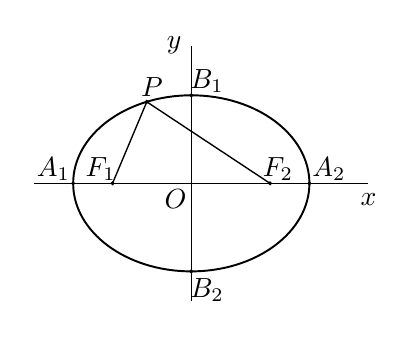
\begin{tikzpicture}[scale=0.5]
      \draw[\myaxisarrow] (-4,0) -- (4.5,0) node[below] {$x$} coordinate(x axis);
      \draw[\myaxisarrow] (0,-3) -- (0,3.5) node[left] {$y$} coordinate(y axis);
      \draw [line width=0.7pt] (0.,0.) ellipse (3 and 2.236);
      \draw [line width=0.5pt] (-2.,0.)-- (-1.13,2.07);
      \draw [line width=0.5pt] (-1.13,2.07)-- (2.,0.);
      
      \draw [fill=black] (-2.,0.) circle (1pt);
      \draw[color=black] (-2.3,0.37) node {$F_1$};
      \draw [fill=black] (2.,0.) circle (1pt);
      \draw[color=black] (2.2,0.37) node {$F_2$};
      \draw [fill=black] (-3.,0.) circle (1pt);
      \draw[color=black] (-3.5,0.37) node {$A_1$};
      \draw [fill=black] (3.,0.) circle (1pt);
      \draw[color=black] (3.5,0.37) node {$A_2$};
      \draw [fill=black] (0,2.236) circle (1pt);
      \draw[color=black] (0.4,2.6) node {$B_1$};
      \draw [fill=black] (0,-2.236) circle (1pt);
      \draw[color=black] (0.4,-2.7) node {$B_2$};
      \draw [fill=black] (-1.13,2.07) circle (1pt);
      \draw[color=black] (-1.,2.45) node {$P$};
      \draw (-0.4,-0.4) node {$O$};
    \end{tikzpicture}
    \caption{}\label{fig-190127-2125}
\end{figure}

再设 $P(x,y)$, 则由两点之间距离公式, 上面的等式化为
\[\sqrt{(x+c)^2+y^2}+\sqrt{(x-c)^2+y^2}= 2a,\]
进一步可以简化为
\[\frac{x^2}{a^2}+\frac{y^2}{a^2-c^2}=1.\]
令 $a^2-c^2=b^2$ ($b>0$), 则得椭圆的标准方程
\[C\colon \frac{x^2}{a^2}+\frac{y^2}{b^2}=1\quad (a>b>0).\]
有时, 椭圆 (ellipse) 也用字母 $E$ 表示. 注意, 上式为焦点在 $x$ 轴上 (``躺着'') 的椭圆的标准方程, 而焦点在 $y$ 轴上 (``立着'') 的椭圆的标准方程形如
\[C'\colon \frac{y^2}{a^2}+\frac{x^2}{b^2}=1\quad (a>b>0).\]
以下只分析前一种椭圆, 对后一种也有类似的结论.

由 $a^2-c^2=b^2$ 知 $a^2=b^2+c^2$, 即 $a$ 值最大. 定义 $e=\dfrac{c}a$ 为椭圆的离心率, 则 $e\in(0,1)$. 离心率 $e$ 的大小表示焦点远离中心的程度: $e$ 越小, 焦点离中心越近, 椭圆越圆; $e$ 越大, 焦点离中心越远, 椭圆越扁. 椭圆 $C$ 的方程表明其为轴对称图形和中心对称图形, 且对称轴为 $x$ 轴和 $y$ 轴, 对称中心为原点, 故原点也称为 $C$ 的中心. 椭圆 $C$ 与 $x$ 轴交于 $A_1(-a,0)$ (左顶点), $A_2(a,0)$ (右顶点), 与 $y$ 轴交于 $B_1(0,b)$ (上顶点), $B_2(0,-b)$ (下顶点). 称线段 $A_1A_2$ 为椭圆 $C$ 的长轴, $B_1B_2$ 为其短轴, 而 $a$, $b$ 分别为长半轴长和短半轴长. 此外还有 $|F_1B_1|=a$.

\lianxi
\begin{exercise}
    已知椭圆 $C\colon \dfrac{x^2}{a^2}+\dfrac{y^2}{b^2}=1$ ($a>b>0$) 的焦距为 $4$, 且过点 $P(\sqrt2,\sqrt3)$, 求椭圆 $C$ 的方程.
\end{exercise}
\beginsolution
    方法一: 半焦距 $c=2$, 则
    \[\left\{\!\!\begin{array}{l}
        \dfrac3{a^2}+ \dfrac3{b^2}= 1,\\
        a^2= b^2+4,
    \end{array}\right.\quad
    \left\{\!\!\begin{array}{l}
        a^2= 8,\\
        b^2= 4.
    \end{array}\right.\]
    椭圆 $C$ 的方程为 $\dfrac{x^2}8+ \dfrac{y^2}4= 1$.

    方法二: 焦点为 $(-2,0)$, $(2,0)$, 则
    \mymarginpar{两种方法计算量差不多, 方法二需要一点配方技巧.}
    \[\begin{aligned}
        2a&= \sqrt{(\sqrt2+2)^2+ (\sqrt3)^2}
            + \sqrt{(\sqrt2-2)^2+ (\sqrt3)^2}\\
        &= \sqrt{9+4\sqrt2}+ \sqrt{9-4\sqrt2}\\
        &= \sqrt{(2\sqrt2+1)^2}+ \sqrt{(2\sqrt2-1)^2}
         = 4\sqrt2,
    \end{aligned}\]
    所以 $a=\sqrt2$, $b=2$, 答案同上.
\endsolution

\begin{exercise}
    “$m>n$”是“方程 $\dfrac{x^2}n +\dfrac{y^2}m =1$ 表示焦点在 $y$ 轴上的椭圆”的什么条件?
\end{exercise}
\beginsolution
    后者等价于 $m>n>0$, 则前者是后者的必要不充分条件.

    \varexercise 若 $\lambda\in (0,1)$, 判断曲线 $C\colon \dfrac{x^2}{\lambda}+ \dfrac{y^2}{1-\lambda}= 1$ 的形状.

    当 $\lambda\in \biggl(0,\dfrac12\biggr)$ 时, 曲线 $C$ 是焦点在 $y$ 轴、中心为原点的椭圆; 当 $\lambda= \dfrac12$ 时, 曲线 $C$ 是原心为原点、半径为 $\dfrac{\sqrt2}2$ 的圆; 当 $\lambda\in \biggl(\dfrac12,1\biggr)$ 时, 曲线 $C$ 是焦点在 $x$ 轴、中心为原点的椭圆.
\endsolution

\begin{exercise}
    已知 $F_1$, $F_2$ 是椭圆 $C\colon \dfrac{x^2}{16}+\dfrac{y^2}{9}=1$ 的两个焦点, 过点 $F_1$ 作倾斜角为 $\alpha$ 的直线与椭圆 $C$ 交于 $A$,$B$ 两点, 求 $\triangle ABF_2$ 的周长.
\end{exercise}
\beginsolution
    由椭圆的定义,
    \[|AF_1|+ |AF_2|= |BF_1|+ |BF_2|= 2\cdot 4= 8,\]
    则$\triangle ABF_2$ 的周长为 $16$.
\endsolution

\begin{exercise}
    若椭圆 $C\colon \dfrac{x^2}{a^2}+\dfrac{y^2}{b^2}=1$ ($a>b>0$) 的离心率为 $\dfrac35$, 两个焦点分别为 $F_1$,$F_2$, $M$ 为椭圆上一点, 且 $\triangle F_1 F_2 M$ 的周长为 16, 求椭圆 $C$ 的方程.
\end{exercise}
\beginsolution
    设半焦距为 $c$, 则
    \[\frac{c}{a}= \frac35,\quad 2a+2c= 16,\]
    解得 $a=5$, $c=3$. 因此 $b=4$, 求椭圆 $C$ 的方程为
    \[\frac{x^2}{25}+\frac{y^2}{16}= 1.\]
\endsolution

\subsection{要点导学\quad 各个击破}
\subsubsection{求椭圆的方程}
\begin{example}
    已知点 $F_1(-1,0)$, $F_2(1,0)$ 是椭圆 $C$ 的两个焦点, 过点 $F_2$ 且垂直于 $x$ 轴的直线交椭圆 $C$ 于 $A$, $B$ 两点, 且 $|AB|=3$, 求椭圆 $C$ 的标准方程.
\end{example}
\beginsolution
    记半焦距 $c=1$, 设椭圆 $C$ 的方程为 $\dfrac{x^2}{a^2}+\dfrac{y^2}{b^2}=1$ ($a>b>0$).

    方法一: 由题意, 可设 $A\biggl(1,\dfrac32\biggr)$, $B\biggl(1,-\dfrac32\biggr)$, 则
    \[2a= |AF_1|+ |AF_2|= \frac52+ \frac32= 4.\]
    所以 $a=2$, $b=\sqrt3$, 椭圆 $C$ 的标准方程为
    \[\frac{x^2}{4}+\frac{y^2}{3}= 1.\]

    方法二: 将 $AB\colon x=c$ 代入椭圆 $C$ 的方程,
    \mymarginpar{线段 $AB$ 称为椭圆 $C$ 的通径, 长度为 $\dfrac{2b^2}a$.}
    \[\frac{c^2}{a^2}+ \frac{y^2}{b^2}= 1,\quad
    y= \pm\frac{b^2}{a},\]
    则 $|AB|= \dfrac{2b^2}a= 3$. 结合 $a^2= b^2+c^2$ 知, $a=2$, $b=\sqrt3$, 答案同上.
\endsolution

\begin{example}
    已知椭圆 $C\colon \dfrac{x^2}{a^2}+\dfrac{y^2}{b^2}=1$ ($a>b>0$) 过点 $A\Big(1,\dfrac32\Big)$, 且离心率 $e=\dfrac12$, 求椭圆 $C$ 的标准方程.
\end{example}
\beginsolution
    设半焦距为 $c$, 则 $\dfrac{c}a= \dfrac12$, 所以 $a=2c$, $b=\sqrt3c$, 连同点 $A\Big(1,\dfrac32\Big)$ 代入椭圆 $C$ 的方程, 得
    \[c=1,\quad a=2,\quad b=\sqrt3.\]
    椭圆 $C$ 的标准方程为
    \[\frac{x^2}{4}+\frac{y^2}{3}= 1.\]
\endsolution

\lianxi
\begin{exercise}
    已知椭圆 $C_1 \colon \dfrac{x^2}4+y^2=1$, 中心在原点的椭圆 $C_2$ 以椭圆 $C_1$ 的长轴为短轴, 且与椭圆 $C_1$ 有相同的离心率, 求椭圆 $C_2$ 的标准方程.
\end{exercise}
\beginsolution
    设椭圆 $C_1$ 的长半轴长、短半轴长、半焦距和离心率分别为 $a_1$,$b_1$,$c_1$ 和 $e_1$, 椭圆 $C_2$ 的长半轴长、短半轴长、半焦距和离心率分别为 $a_2$,$b_2$,$c_2$ 和 $e_2$, 则
    \mymarginpar{离心率相同, 则对应线段成比例.}
    \[a_1=2,\ b_1= 1,\ c_1= \sqrt3,\quad
    b_2= a_1= 2,\ e_2=e_1= \frac{\sqrt3}{2},\]
    所以 $a_2= 4$, 椭圆 $C_2$ 的标准方程为
    \[\frac{x^2}{16}+\frac{y^2}{4}= 1.\]
\endsolution

\begin{exercise}
    若椭圆 $C\colon \dfrac{x^2}{a^2}+\dfrac{y^2}{b^2}=1$ ($a>b>0$) 的离心率 $e=\dfrac{\sqrt3}2$, $a+b=3$, 求椭圆 $C$ 的方程.
\end{exercise}
\beginsolution
    设半焦距为 $c$, 则 $\dfrac{c}a= \dfrac{\sqrt3}2$, 可设
    \mymarginpar{由比例式设参数 $k$ 可以简化计算.}
    \[a= 2k,\ c=\sqrt3 k,\quad k>0,\]
    此时 $b=k$, 且
    \[a+b= 2k+k= 3,\quad k=1.\]
    所以 $a=2$, $b=1$, 椭圆 $C_2$ 的标准方程为
    \[\frac{x^2}4+ y^2= 1.\]
\endsolution

\subsubsection{椭圆定义的应用}
\begin{example}
    已知 $\triangle ABC$ 的三边长 $a$,$b$,$c$ ($a>b>c$) 成等差数列, $A(-1,0)$, $C(1,0)$, 求点 $B$ 的轨迹.
\end{example}
\beginsolution
    $a+c= 2b$, 即
    \mymarginpar{这里的 $a$,$b$,$c$ 并不是椭圆的长半轴长、短半轴长、半焦距.}
    \[|BC|+ |BA|= 2|AC|= 4,\]
    则点 $B$ 在椭圆 $E\colon \dfrac{x^2}4+ \dfrac{y^2}3= 1$ 上. 由 $a>c$ 即 $|BC|> |BA|$ 知, 点 $B$ 的轨迹为椭圆 $E$ 在 $y$ 轴左侧的部分, 且不含左顶点 $(-2,0)$. 
\endsolution

\lianxi
\begin{exercise}
    已知中心为原点、左焦点为 $F(-1,0)$ 的椭圆 $C$ 过点 $A\biggl(1,\dfrac{2\sqrt3}3\biggr)$, 求椭圆 $C$ 的标准方程.
\end{exercise}
\beginsolution
    右焦点 $F'(1,0)$, 长轴长
    \mymarginpar{也可以将点 $A$ 的坐标代入椭圆 $C$ 的标准方程来求解.}
    \[2a= |AF|+|AF'|= 2\sqrt3,\]
    则 $a= \sqrt3$, 短半轴长 $b=\sqrt2$. 椭圆 $C$ 的标准方程为
    \[\frac{x^2}3+ \frac{y^2}2= 1.\]
\endsolution

\begin{exercise}
    已知椭圆 $C\colon \dfrac{x^2}{a^2}+\dfrac{y^2}{b^2}=1$ ($a>b>0$) 的左顶点为 $A$, 左焦点为 $F$, 上顶点为 $B$. 若 $\angle BAO+\angle BFO=90^\circ$, 求椭圆 $C$ 的离心率.
\end{exercise}
\beginsolution
    由题意, $\angle BAO= \angle FBO$, 则
    \[\tan\angle BAO= \tan\angle FBO,\quad 
    \frac{b}a= \frac{c}b,\]
    则 $b^2= ac= a^2-c^2$. 同除以 $a^2$ 得,
    \[e^2+e-1=0,\quad e=\frac{\sqrt5-1}{2}.\]
\endsolution

\subsubsection{椭圆与直线相交}
\begin{example}
    设点 $A_1$,$A_2$ 与 $B$ 分别是椭圆 $E\colon \dfrac{x^2}{a^2}+\dfrac{y^2}{b^2}=1$ ($a>b>0$) 的左顶点、右顶点与上顶点, 直线 $A_2 B$ 与圆 $C\colon x^2+y^2 =1$ 相切. 若直线 $l$ 与椭圆 $E$ 交于 $M$,$N$ 两点, 且 $\overrightarrow{OM}\cdot \overrightarrow{ON}=0$, 试判断直线 $l$ 与圆 $C$ 的位置关系, 并说明理由.
\end{example}
\beginsolution
    $A_2(a,0)$, $B(0,b)$, 则
    \[AB\colon \frac{x}a+ \frac{y}b= 1,\ \text{即}\ 
    bx+ay-ab=0.\]
    由题意, 点 $C(0,0)$ 到直线 $A_2B$ 的距离为圆 $C$ 的半径 $r=1$, 则
    \[\frac{|-ab|}{\sqrt{b^2+a^2}}= 1,\quad
    a^2+b^2= a^2b^2.\]

    (1) 若直线 $l$ 的斜率不存在, 由 $\overrightarrow{OM}\cdot \overrightarrow{ON}=0$ 知, $\triangle MON$ 为等腰直角三角形, 且点 $O$ 为直角顶点. 可设 $N(n,n)$, 代入椭圆 $E$ 的方程知, 
    \[\frac{n^2}{a^2}+ \frac{n^2}{b^2}= 1,\quad n= \pm1,\]
    表明直线 $l$ 与圆 $C$ 相切.

    (2) 若直线 $l$ 的斜率存在, 设 $l\colon y=kx+m$ 并代入椭圆 $E$ 的方程,
    \[(b^2+ a^2 k^2)x^2+ 2a^2mkx+ a^2(m^2-b^2)= 0.\]
    设 $M(x_1,y_1)$, $N(x_2,y_2)$, 则
    \[x_1+x_2= -\frac{2a^2mk}{b^2+ a^2 k^2},\quad
    x_1x_2= \frac{a^2(m^2-b^2)}{b^2+ a^2 k^2}.\]
    由 $\overrightarrow{OM}\cdot \overrightarrow{ON}=0$ 知, $x_1x_2+y_1y_2= 0$, 即
    \[\begin{gathered}
        (1+k^2)x_1x_2+ mk(x_1+x_2)+ m^2= 0,\\
        (a^2+b^2)m^2= a^2b^2(1+k^2).
    \end{gathered}\]
    再求点 $C(0,0)$ 到直线 $l$ 的距离
    \[d= \frac{|m|}{\sqrt{1+k^2}}= \sqrt{\frac{a^2b^2}{a^2+b^2}}=1,\]
    此时直线 $l$ 仍与圆 $C$ 相切.
\endsolution

\lianxi
\begin{exercise}[s]
    已知点 $A(0,-2)$, 椭圆 $E\colon \dfrac{x^2}{a^2}+\dfrac{y^2}{b^2}=1$ ($a>b>0$) 的离心率 $e=\dfrac{\sqrt3}2$, $F$ 是椭圆 $E$ 的右焦点, 直线 $AF$ 的斜率为 $\dfrac{2\sqrt3}3$, $O$ 为坐标原点.
    
    (1) 求椭圆 $E$ 的方程;\qquad
    (2) 设过点 $A$ 的动直线 $l$ 与椭圆 $E$ 相交于 $P$,$Q$ 两点, 且 $l$ 与 $x$ 轴不垂直. 用直线 $l$ 的斜率 $k$ 表示 $\triangle OPQ$ 的面积.
\end{exercise}
\beginsolution
    (1) 设半焦距为 $c$, 则 $F(c,0)$,
    \[e= \frac{c}a= \frac{\sqrt3}2,\quad
    \frac{0-(-2)}{c-0}= \frac{2\sqrt3}3,\]
    解得 $c=\sqrt3$, $a=2$, 则 $b=1$. 椭圆 $E$ 的方程为
    \[\frac{x^2}4+ y^2= 1.\]

    (2) 将直线 $l\colon y=kx-2$ 代入椭圆 $E$ 的方程,
    \[(1+4k^2)x^2- 16kx+ 12=0.\]
    设 $P(x_1,y_1)$, $Q(x_2,y_2)$, 则
    \[\begin{aligned}
        |PQ|
        &= \sqrt{1+k^2}|x_1-x_2|
         = \sqrt{1+k^2}\frac{\sqrt{\Delta}}{1+4k^2}\\
        &= \frac{4\sqrt{1+k^2}\sqrt{4k^2-3}}{1+4k^2},\quad
        4k^2>3,
    \end{aligned}\]
    点 $O$ 到直线 $l$ 的距离 $d= \dfrac2{\sqrt{1+k^2}}$, 所以 $\triangle OPQ$ 的面积
    \[S_{\triangle OPQ}= \frac12|PQ|\cdot d
     = \frac{4\sqrt{4k^2-3}}{1+4k^2}.\]
\endsolution

\subsubsection{课堂评价}
\begin{exercise}
    设 $A(-2,0)$, $B(2,0)$, 动点 $P$ 满足直线 $PA$,$PB$ 的斜率之积为 $-\dfrac14$, 求点 $P$ 的轨迹方程.
\end{exercise}
\beginsolution
    设 $P(x,y)$ ($x\neq \pm2$), 则
    \[\frac{y-0}{x+2}\cdot \frac{y-0}{x-2}= -\frac14,\quad
    \frac{x^2}4+y^2= 1\quad (x\neq \pm2).\]
\endsolution

\begin{exercise}
    已知椭圆 $E\colon \dfrac{x^2}{a^2}+\dfrac{y^2}{b^2}=1$ ($a>b>0$) 的离心率为 $\dfrac{\sqrt3}2$, 左焦点、右焦点分别为 $F_1$,$F_2$. 点 $P$ 是椭圆 $E$ 上一点, 且 $\angle F_1PF_2= 90^\circ$, $\triangle F_1PF_2$ 的面积 $S_{\triangle F_1PF_2}= 3$, 求椭圆 $E$ 的方程.
\end{exercise}
\beginsolution
    设半焦距为 $c$, 则 $\dfrac{c}a= \dfrac{\sqrt3}2$, 可设
    \[a=2k,\ c=\sqrt3k,\quad k>0,\]
    则 $b=k$. 再设 $|PF_1|= m$, $|PF_2|= n$, 则
    \[\begin{gathered}
        m+n= 2a= 4k,\quad \frac12mn=3,\quad
        m^2+n^2= (2c)^2= 12k^2.
    \end{gathered}\]
    结合 $(m+n)^2$ 的展开式可解得 $k=\sqrt3$. 椭圆 $E$ 的方程为
    \[\frac{x^2}{12}+ \frac{y^2}{3}= 1.\]
\endsolution

\begin{exercise}
    设直线 $l_1\colon y=-x+1$ 与椭圆 $C\colon \dfrac{x^2}{a^2}+\dfrac{y^2}{b^2}=1$ ($a>b>0$) 相交于 $A$,$B$ 两点, 且线段 $AB$ 的中点 $M$ 在直线 $l_2\colon x-2y=0$ 上, 求椭圆 $C$ 的离心率.
\end{exercise}
\beginsolution
    将 $l_1\colon y=-x+1$ 代入椭圆 $C$ 的方程,
    \[(a^2+b^2)x^2- 2a^2x+ a^2-a^2b^2= 0.\]
    由题意, 点 $M$ 为直线 $l_1$,$l_2$ 的交点 $\biggl(\dfrac23,\dfrac13\biggr)$. 设 $A(x_1,y_1)$, $B(x_2,y_2)$, 则
    \[x_1+x_2= 2\cdot \frac23= \frac{2a^2}{a^2+b^2},\]
    所以 $a=\sqrt2b$. 设半焦距为 $c$, 则由 $a^2= b^2+c^2$ 知 $b=c$, 故离心率 $e= \dfrac{c}a= \dfrac{\sqrt2}2$.
\endsolution

\subsection{课后练习}

\begin{exercise}
    已知椭圆 $C\colon \dfrac{x^2}{a^2}+\dfrac{y^2}{b^2}=1$ ($a>b>0$) 的焦距为 $4$, 其短轴的两个端点与长轴的一个端点构成正三角形, 求椭圆 $C$ 的方程.
\end{exercise}
\beginsolution
    设半焦距为 $c$, 则 $c=2$. 由题意, $a=\sqrt3 b$, 而 $a^2=b^2+c^2$, 所以 $b^2= 2$, $a^2= 6$. 椭圆 $C$ 的方程为
    \[\frac{x^2}{6}+ \frac{y^2}{2}= 1.\]
\endsolution

\begin{exercise}
    已知椭圆 $C\colon \dfrac{x^2}{a^2}+\dfrac{y^2}{b^2}=1$ ($a>b>0$) 的左焦点、右焦点分别为 $F_1$,$F_2$, 离心率 $e= \dfrac{\sqrt3}3$, 过点 $F_2$ 的直线 $l$ 交椭圆 $C$ 于 $A$, $B$ 两点. 若 $\triangle AF_1 B$ 的周长为 $4\sqrt3$, 求椭圆 $C$ 的方程.
\end{exercise}
\beginsolution
    设半焦距为 $c$, 则 
    \[e= \frac{c}a= \frac{\sqrt3}{3},\quad
        4a= 4\sqrt3,\]
    所以 $a=\sqrt3$, $c=1$, $b=\sqrt2$. 椭圆 $C$ 的方程为
    \[\frac{x^2}{3}+ \frac{y^2}{2}= 1.\]
\endsolution

\begin{exercise}
    已知椭圆 $C\colon \dfrac{x^2}{a^2}+\dfrac{y^2}{b^2}=1$ 
    ($a>b>0$), 以 $O$ 为圆心、短半轴长为半径作圆 $O$, 
    过椭圆的右顶点 $P$ 作圆 $O$ 的两条切线, 切点为 $A$, $B$. 
    若 $|AO|= |AP|$, 椭圆 $C$ 的离心率.
\end{exercise}
\beginsolution
    由题意, 四边形 $PAOB$ 为正方形, $a=\sqrt2b$. 因为 $a^2= b^2+c^2$, 所以 $b= c$, 离心率 $e= \dfrac{c}a= \dfrac{\sqrt2}2$.
\endsolution

\begin{exercise}
    已知椭圆 $C\colon \dfrac{x^2}{a^2}+\dfrac{y^2}{b^2}=1$ 
    ($a>b>0$) 的左焦点、右焦点分别为 $F_1$,$F_2$, 圆 $F_2$ 过椭圆 $E$ 的中心, 且与椭圆 $E$ 交于一点 $P$. 若直线 $PF_1$ 与圆 $F_2$ 相切, 求椭圆 $E$ 的离心率.
\end{exercise}
\beginsolution
    设半焦距为 $c$, 则
    \[|PF_2|= c,\quad |PF_1|= 2a-c,\quad |F_1F_2|= 2c.\]
    由题意, $PF_1\perp PF_2$, 则
    \[\begin{gathered}
        |PF_1|^2+ |PF_2|^2= |F_1F_2|^2,\\
        c^2+2ac-2a^2= 0.
    \end{gathered}\]
    两边同除以 $a^2$, 得离心率 $e$ 满足
    \[e^2+2e-2= 0,\quad e= \sqrt3-1.\]
\endsolution

\begin{exercise}
    过点 $M(1,1)$ 作斜率为 $-\dfrac12$ 的直线 $l$ 与椭圆 $C\colon \dfrac{x^2}{a^2}+\dfrac{y^2}{b^2}=1$ ($a>b>0$) 相交于点 $A$,$B$. 若 $M$ 是线段 $AB$ 的中点, 求椭圆 $C$ 的离心率.
\end{exercise}
\beginsolution
    将 $l\colon y-1= -\dfrac12(x-1)$ 代入椭圆 $C$ 的方程, 消去 $x$ 得,
    \[(a^2+4b^2)y^2- 12b^2y+ 9b^2-a^2b^2= 0.\]
    设 $A(x_1,y_1)$, $B(x_2,y_2)$, 则
    \[\frac{y_1+y_2)}{2}= 1,\quad
    y_1+y_2= \frac{12b^2}{9b^2-a^2b^2},\]
    所以 $a=\sqrt2b$. 结合 $a^2= b^2+c^2$ 知 $b=c$, 故离心率为 $\dfrac{\sqrt2}2$.
\endsolution

\begin{exercise}
    设 $F_1$,$F_2$ 分别是椭圆 $E\colon x^2+\dfrac{y^2}{b^2}=1$ ($0<b<1$) 的左焦点、右焦点, 过点 $F_1$ 的直线交椭圆 $E$ 于 $A$, $B$ 两点. 若 $|AF_1| =3|BF_1|$, $AF_2\perp x$ 轴, 求椭圆 $E$ 的方程.
\end{exercise}
\beginsolution
    长半轴长 $a=1$, 设半焦距为 $c$, 则
    \[A\biggl(c,\frac{b^2}{a}\biggr)= (c,b^2),\quad
        F_1(-c,0).\]
    又设 $B(m,n)$, 由题意作图可知, $\overrightarrow{AF_1}= 3\overrightarrow{F_1B}$, 即
    \[\begin{gathered}
        (-c-c,0-b^2)= 3(m+c,n),\\
        m= -\frac{5c}{3},\quad n= -\frac{b^2}{3},
    \end{gathered}\]
    代入椭圆 $E$ 的方程, 并结合 $b^2+c^2=a^2=1$, 解得 $b^2= \dfrac23$. 椭圆 $E$ 的方程为
    \[x^2+ \frac{3y^2}{2}= 1.\]
\endsolution

\begin{exercise}
    已知椭圆 $C$ 经过点 $M(4,1)$, 中心在原点, 焦点在 $x$ 轴上, 离心率为 $\dfrac{\sqrt3}2$. 若直线 $l\colon y=x+m$ 交椭圆 $C$ 于不同的两点 $A$,$B$, 求实数 $m$ 的取值范围.
\end{exercise}
\beginsolution
    设椭圆 $C$ 的标准方程为
    \[\frac{x^2}{a^2}+ \frac{y^2}{b^2}=1\quad (a>b>0),\]
    且半焦距为 $c$, 则
    \[\frac{c}{a}= \frac{\sqrt3}{2},\quad
    \frac{16}{a^2}+ \frac{1}{b^2}=1,\]
    结合 $b^2+c^2=a^2$ 解得 $b^2= 5$, $a^2= 20$. 将 $l\colon y=x+m$ 代入椭圆 $C$ 的方程,
    \[\begin{gathered}
        5x^2+ 8mx+ 4m^2-20= 0,\\
        \Delta= (8m)^2- 4\cdot 5(4m^2-20)>0,
    \end{gathered}\]
    所以 $m\in (-5,5)$.
\endsolution

\begin{exercise}
    已知椭圆 $E\colon \dfrac{x^2}{a^2}+y^2= 1$ ($a>0$) 的右顶点为 $A$, 左顶点为 $B$, 上顶点为 $G$, $\overrightarrow{AG}\cdot \overrightarrow{GB}= 8$. 动点 $P$ 在直线 $x=6$ 上, 直线 $PA$,$PB$ 分别与椭圆 $E$ 交于点 $C$,$D$.

    (1) 求椭圆 $E$ 的方程;\qquad (2) 证明: 直线 $CD$ 过定点.
\end{exercise}
\beginsolution
    (1) 由题意, $A(-a,0)$, $B(a,0)$, $G(0,1)$, 则
    \[\overrightarrow{AG}\cdot \overrightarrow{GB}
    = (a,1)\cdot (a,-1)= 8,\]
    解得 $a=3$, 所以椭圆 $E$ 的方程为
    \[\dfrac{x^2}9+ y^2= 1.\]

    (2) 设 $P(6,p)$, 由 $A(-3,0)$ 知
    \[PA\colon y= \frac{p}{9}(x+3),\]
    代入椭圆 $E$ 的方程,
    \[(9+p^2)x^2+ 6p^2x+ 9p^2-81= 0.\]
    设 $C(x_C,y_C)$, 则
    \[\begin{gathered}
        x_C\cdot (-3)= \frac{9p^2-81}{9+p^2},\\
        x_C= \frac{27-3p^2}{9+p^2},\quad
        y_C= \frac{6p}{9+p^2}.
    \end{gathered}\]
    设 $D(x_D,y_D)$, 则同理可得,
    \[x_D= \frac{3p^2-3}{1+p^2},\quad
        y_D= \frac{-2p}{1+p^2}.\]
    由对称性知, 若 $CD$ 过定点 $Q(x_Q,y_Q)$, 则点 $Q$ 必在 $x$ 轴上.
    \mymarginpar{利用对称性判断定点的位置, 可以简化计算.}

    若 $x_C= x_D$, 则 $p^2= 3$, 而 $x_C= \dfrac32$, 所以直线 $CD\colon x=\dfrac32$, 表明定点 $Q$ 只能为 $\biggl(\dfrac32,0\biggr)$.

    若 $x_C\neq x_D$, 则直线 $CQ$,$DQ$ 的斜率分别为
    \mymarginpar{也可以由两点式得到 (计算量较大)
    \[CD\colon 3\biggl(p-\frac3p\biggr)y+4x=6,\]
    也表明直线 $CD$ 过定点 $\biggl(\dfrac32,0\biggr)$.}
    \[\begin{aligned}
        k_{CQ}&= \frac{y_C- y_Q}{x_C- x_Q}
            = \frac{\dfrac{6p}{9+p^2}- 0}{
                \dfrac{27-3p^2}{9+p^2}- \dfrac32}
            = \frac{4p}{9-3p^2},\\
        k_{DQ}&= \frac{y_D- y_Q}{x_D- x_Q}
            = \frac{\dfrac{-2p}{1+p^2}- 0}{
                \dfrac{3p^2-3}{1+p^2}- \dfrac32}
            = \frac{4p}{9-3p^2},
    \end{aligned}\]
    表明直线 $CD$ 仍过点 $Q$.
\endsolution
